\section{Fazit}
\label{sec:conclusion}

Die in Kapitel \ref{sec:requirements} beschriebenen Ziele wurden grundsätzlich erreicht:
Schüler können neue Bilder in Ihre Projekte einpflegen (und diese auch verwenden).
Außerdem wurden die Kompilierungsschritte in einer weitestgehend
platformunabhängigen Docker-Umgebung gekapselt. Dieses Kapitel fasst zusammen
inwiefern die jeweiligen Implementierungen vollständig sind und gibt einen Ausblick
auf mögliche Erweiterungen.

\subsection{Erreichte Ziele}

Es wurde eine einheitliche Umgebung geschaffen um die Rails und Angular
Toolchain zu Betreiben. Wie in Kapitel \ref{subsec:4-containerization} erläutert,
wurde eine Umgebung für die Verwendung durch Entwickler zum ausführen der
Anwendung im Entwicklungsmodus sowie eine zum automatisierten Ausführen der
Tests.

Weiterhin wurde wie in Kapitel \ref{subsec:4-image-library} ff. ein Prototyp einer
Bildverwaltung implementiert, der es Erlaubt dem Projektautoren Bilder für die
Nutzung innerhalb des Projekts hochzuladen und sowohl als statische Inhalte im
Seiteneditor zu verwenden, als Ergebnis von Datenbankabfragen zu rendern. Bilder
die als Ergebnis einer Datenbankabfrage gerendert werden, werden im Footer der
Seite mit Urheber und Lizenz aufgeführt, sowie alle nicht als Figure Umgebung
angezeigten statischen Bilder. Bei Figure Umgebungen werden die Angaben zu
Urheber und Lizenz zusammen mit dem Bildtitel direkt unter dem Bild angezeigt.
Abbildung \ref{fig:wiki-article} zeigt beide Verwendungsmöglichkeiten von
statischen Bildern, während Kapitel \ref{sec:introduction} bereits in Abbildung
\ref{fig:comparison-after} die Verwendung von Bildern im Ergebnis einer
Datenbankabfrage gezeigt hat.

\begin{figure}
  \centering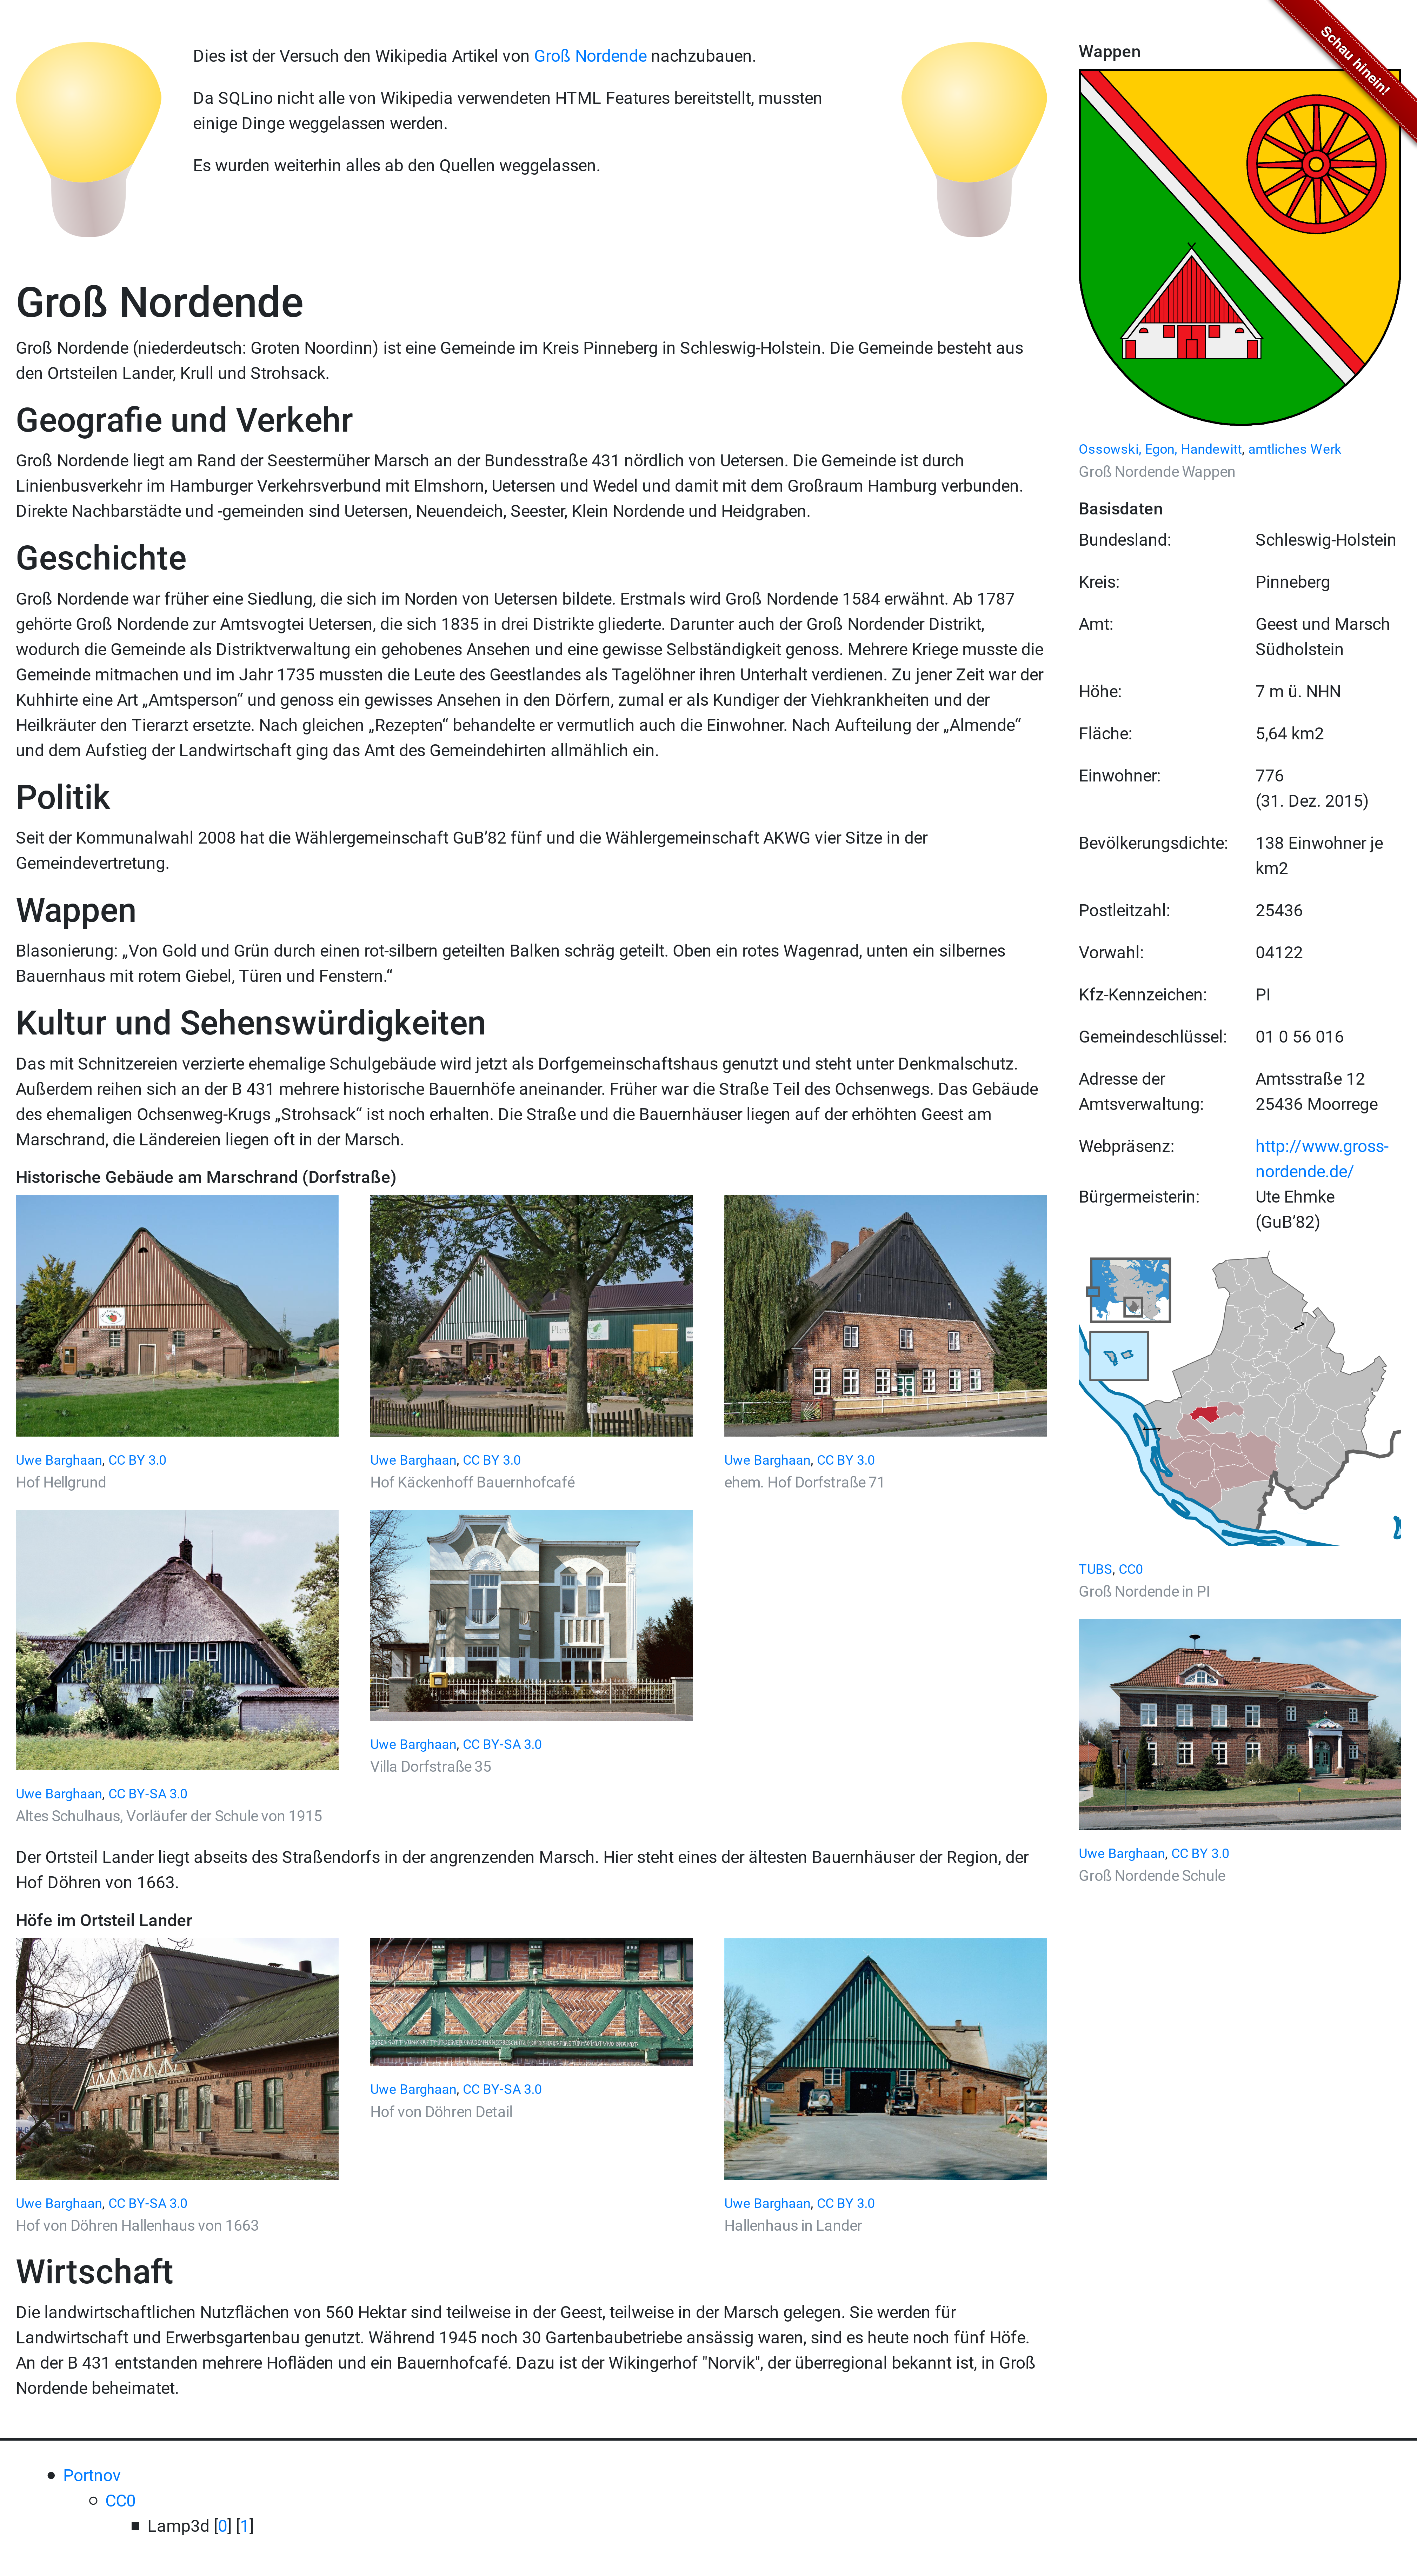
\includegraphics[height=0.95\textheight]{images/conclusion-example-wikipage.png}
  \caption{Nachbau eines Wikipedia Artikels in SQLino}
  \label{fig:wiki-article}
\end{figure}

\subsection{Nicht erreichte Ziele}

Die Urprünglichen Ziele konnten aufgrund einiger unerwarteter Untiefen im Umfang
der Umsetzung nicht erreicht werden. Offen geblieben sind
\begin{description}
  \item[Import aus Bilddatenbanken] \mbox{} \\ Import mit Suche für Bilder mit
    passender Lizenz in öffentlichen Bilddatenbanken, bei dem alle benötigen
    Metadaten automatisch importiert werden.
  \item[Projektübergreifende Bildverwaltung] \mbox{} \\ Administrator geführte
    Bildverwaltung, in der projektübergreifend Bilder abgelegt und von allen
    Projekten verwendet werden können.
  \item[Administrator Interface] \mbox{} \\ Ein Interface für den
    Systemadministrator/Lehrer um Projektübergreifend nach Bildern zu suchen und
    diese zu sperren, sowie Anträge auf Weglassen der Quellenangabe bei eigenen
    Werken zu bestätigen.
  \item[Einstellbare Darstellungsoptionen] \mbox{} \\ Zuätzlichen
    konfigurierbare Bildeigenschaften im Seiteneditor, um die Möglickeiten der
    Seitengestaltung zu erweitern.
  \item[Produktivumgebung] \mbox{} \\ Die vereinheitlichte Umgebung für den
    Produktivbetrieb von SQLino.
\end{description}

Kapitel \ref{subsec:3-image-library} geht darauf ein, weshalb der Bildupload pro
Projekt höher priorisiert wurde, als die nicht umgesetzen Varianten des Imports
aus öffentlichen Bilddatenbanken und der Zentralen Bilddatenbank. Natürlich ist
die Umsetzung aller drei wünschenswert, muss aus zeitlichen Gründen aber später
erfolgen.

Das Interface zum Bilder sperren ist zwar notwendig, bevor SQLino produktiv
genutzt werden kann, setzt allerdings die vorherige Umsetzung der erreichten
Ziele voraus, weshalb diese vorrangig behandelt wurden.

Wie im Kapitel \ref{subsec:4-page-editor} dargelegt konnten nicht alle Features für
den Seiteneditor umgesetzt werden, weshalb dort nur ihr Sollzustand beschrieben
ist. Die aktuelle Implementierung erlaubt es nicht, die Dimensionen der
dargestellten Bilder im Seiteneditor festzulegen, daher werden alle Bilder immer
mit maximaler Größe dargestellt. Diese ergibt sich aus der Breite des umgebenden
Elements der Seite sowie bei Rastergrafiken aus der Auflösung, in der das Bild
vorliegt, daher ist die derzeit einzige Möglichkeit ein Bild kleiner als über
die gesamte Breite der Seite darzustellen die Verwendung der \texttt{row} und
\texttt{col} Elemente des Seiteneditors zur Beschränkung der Bildbreite. Derzeit
ist es nicht möglich beispielsweise Pixelart groß darzustellen, ohne sie mit
einem Grafikeditor zu skalieren und der Bildverwaltung in dieser Version
hinzuzufügen. Weiterhin fehlt die Möglichkeit ein Bild von Text umfließen zu
lassen.

Da SQLino noch nicht den Stand des Produktivbetriebs erreicht hat, war die
Priorität der einheitlichen Produktivumgebung, die eine direkt lauffähige
Instanz von SQLino bereitstellt hinten angestellt und dementsprechend nicht
vollendet. Allerdings sind diverse dafür notwendige Schritte analog zu der
Entwicklungs und Testumgebung, allerdings mit anderer Konfiguration.

\subsection{Weiterentwicklung}

Nach der geplanten Umstellung der Datenbaken von SQLite auf PostgreSQL ist es
sinnvoll die Metadaten der Bilder nicht mehr in einer eigenen Datei auf der
Festplatte zu speichern, sondern in der Datenbank, da zum einen die Datenbank
problemlos auf einen anderen Server ausgelagert werden kann, als auch aus
Programmierer Sicht eine Vereinfachung für die Implementierung der geplanten
Projektvererbung. Dies ermöglicht außerdem der Datenbank die Abfragen nach den
Bildern im Cache vorzuhalten und so erneute Abfragen zu beschleunigen. Für die
Datenbank würde zumindest in der Produktiv- und Entwicklungsvariante ein
dedizierter Container zum Einsatz kommen, der im Fall von PostgreSQL bereits in
mehreren Varianten auf Dockerhub zur Verügung steht.

%%% Local Variables:
%%% mode: latex
%%% TeX-master: "thesis"
%%% End:
